\chapter{Estado da arte}

\section{\textit{Structure from motion}}

\textit{Structure from motion} é o processo de estimar estruturas 3D partindo de imagens sequenciais em duas dimensões \cite{SFM}, que pode conter sinais de movimento, em analogia com a biologia, seria o equivalente ao modo  como os olhos humanos e de outros animais conseguem recuperar estruturas 3D de um plano 2D, nesse caso a retina, partindo de uma cena ou objeto em movimento.

Tendo como exemplo os planos $C$ e $C'$ na equação \eqref{eq1} , dois pontos, chamados $m$ no plano $C$ e $m'$ no plano $C'$, podem ser chamados de correspondentes se há projeções do mesmo ponto 3D no espaço $M$. Havendo mais de uma imagem, algumas perguntas podem ser feitas, como:

\begin{itemize}
	\item{Dado um ponto m na primeira imagem, onde está seu correspondente m’ na segunda imagem?}
	\item{Qual a geometria 3D da cena?}
	\item{Qual a posição relativa de ambas câmeras?}
\end{itemize}
	
Com pelo menos duas imagens em diferentes posições, se torna possível inferir a posição 3D de um ponto utilizando sua diferença de posição em ambas imagens. Para tanto é necessário deduzir a posição de duas retas num sistema de coordenadas em comum e é preciso também ter conhecimento da posição relativa da segunda imagem ou câmera com a primeira, o que pode ser chamado de movimento.

Algebricamente, é possível descrever as características da câmera em matrizes chamadas \textbf{matrizes de projeção} \cite{Faugeras-Geometry} com as quais, sabendo seus valores, obtém-se um sistema de equações e computa-se o plano $M$, abaixo:

 \begin{equation}\label{eq1}
	\begin{bmatrix}
		P
	\end{bmatrix}
	\begin{bmatrix}
		x\\y\\z
	\end{bmatrix}
	\begin{bmatrix}
		m\\v\\1
	\end{bmatrix}
	\begin{bmatrix}
		m'\\v'\\1
	\end{bmatrix}
\end{equation}	
 

Equação \eqref{eq1} : Matriz de projeção $P$, plano $M$ e retas $m^T = \begin{bmatrix}u & v & 1\end{bmatrix}$ e $m'^T = \begin{bmatrix}u' & v' & 1\end{bmatrix}$, respectivamente.

\begin{equation}\label{eq2}
\begin{cases}
P M \simeq m, \\
P' M \simeq m'.
\end{cases}
\end{equation}

Equação \eqref{eq2} : Sistema de equações para a matriz de projeção $P$ e $P'$, respectivamente.

Para encontrar a estrutura 3D da cena, é necessário obter as matrizes de projeção $P$ e $P'$, pois possuem informações acerca da geometria da cena. As equações da figura 2.2 representam o sistema com três incógnitas e para que seja possível uma solução, as coordenadas de $m$ e $m'$ precisam satisfazer algumas restrições, logo, o ponto $m'$ não pode ser um ponto arbitrário na segunda imagem.

Seja um exemplo em que os pontos 3D estejam num plano II, havendo uma homografia \cite{Faugeras-Geometry} entre II e cada uma das imagens, pode-se concluir que há uma homografia entre ambas imagens, chamada \textbf{homografia planar}, definida por uma matriz 3x3 $M$. Tal homografia é exemplificada como equação pela equacão \eqref{eq3} e também na figura \ref{fig1}:

\begin{equation}\label{eq3}
m' \simeq Hm.
\end{equation}

Equação \eqref{eq3} : Relação de homografia entre um ponto $m'$ da segunda imagem com um ponto $m$ da primeira, como equação.

\begin{figure}
	\centering
		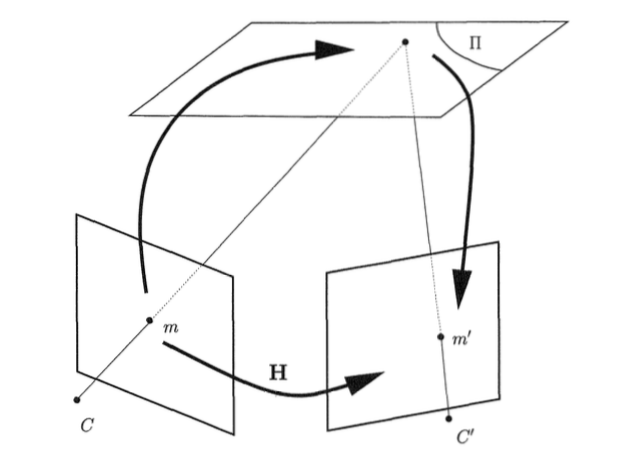
\includegraphics{Imagens/figura2-1.png}
	\caption{Relação de homografia entre um ponto $m'$ da segunda imagem com um ponto $m$ da primeira. Faugeras et al [2] pag. 22.}
	\label{fig1}
\end{figure}

Um outro caso que vale frisar é quando os centros ópticos de ambas imagens são o mesmo, como por exemplo, quando tiradas do mesmo ponto mas apenas com uma rotação. Sejam $m$ e $m'$ pontos arbitrários da imagem 1 e 2, respectivamente, para qualquer plano II que não passe pelo centro ótico das imagens, as imagens também são pontos de interseção dos raios em comum de ambas. Portanto, são relacionadas pela matriz $H$. Tal homografia pode ser utilizada para construir mosaicos, como mostra a figura \ref{fig2} abaixo. Aplicando na primeira imagem, transformando numa imagem maior representando a cena pelo ponto de vista da segunda imagem mas com uma área de visão maior. Apesar de conseguir gerar um campo de visão maior, não é possível obter coordenadas 3D à partir de imagens com o mesmo centro óptico \cite{Faugeras-Geometry}, pois a ambiguidade continua já que os raios correspondentes são idênticos.

\begin{figure}
	\centering
		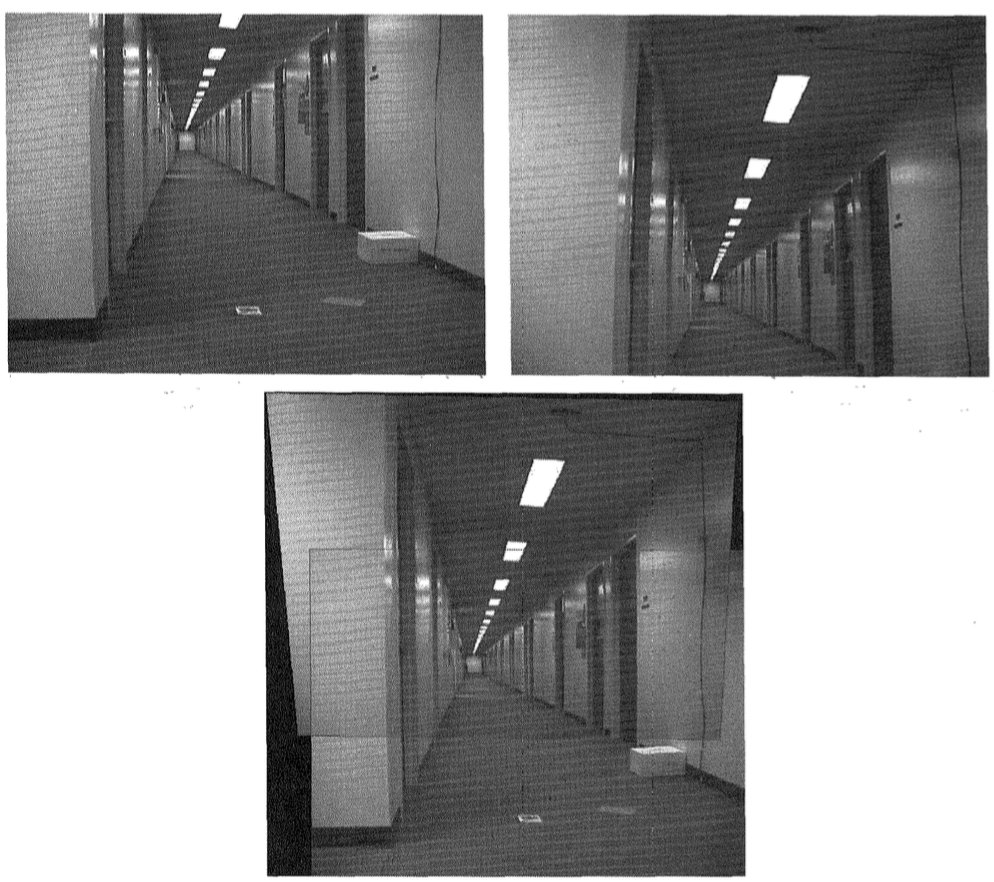
\includegraphics[width=1.0\textwidth]{Imagens/figura2-2.png}
	\caption{Duas imagens obtidas com o mesmo ponto de vista, e a imagem resultante da junção das duas com homografia. Faugeras et al \cite{Faugeras-Geometry} pag. 24.}
	\label{fig2}
\end{figure}

Quando os pontos no espaço e as duas câmeras estão em posições distintas, não é possível predizer a posição do correspondente $m'$ de um ponto qualquer $m$ da primeira imagem, pois tal informação depende da profundidade do ponto 3D ao longo do raio óptico. Geometricamente tal posição não é arbitrária, tal ponto $m$ precisa estar numa linha, o raio óptico, logo $m'$ precisa estar localizado na projeção da reta na segunda imagem. Tal linha é chamada \textbf{Linha Epipolar}, do ponto \textbf{m} na segunda imagem. Tendo conhecimento dela, ao procurar o correspondente $m'$, não é necessário procurar em toda a imagem, bastando apenas na linha, reduzindo então uma busca 2D para 1D, mostrado na figura \ref{fig3}.

\begin{figure}
	\centering
		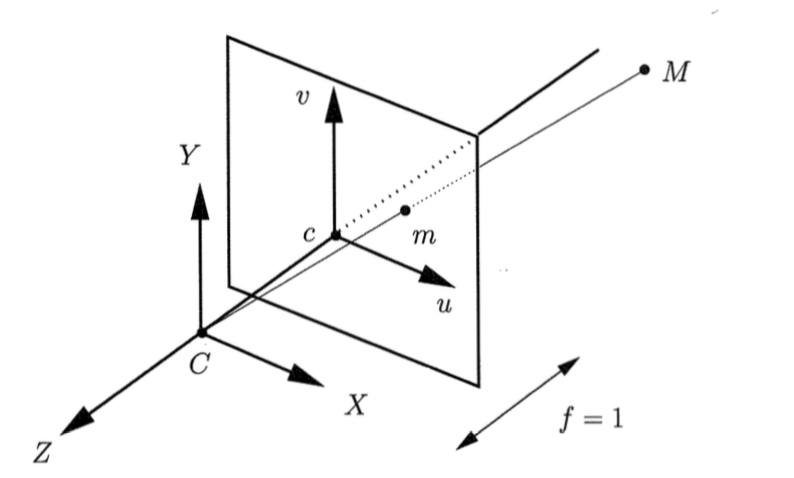
\includegraphics{Imagens/figura2-3.png}
	\caption{Exemplificação da redução de 2D para 1D. Faugeras et al \cite{Faugeras-Geometry} pag. 12.}
	\label{fig3}
\end{figure}

Outra forma de se obter o mesmo resultado é considerar algumas restrições às câmeras ao invés de sua correspondência. Supondo que há uma correspondência válida entre $m$ e $m'$, a posição relativa de ambas as câmeras precisa ser de forma que os raios ópticos $Lm$ e $Lm'$ se interceptem. Algebricamente, já que o ponto $M$ da figura \ref{eq2} depende de três coordenadas, e a correspondência entre $m$ e $m'$ depende no total de 4 parâmetros, é necessário também que haja uma relação algébrica entre as coordenadas de $m$ e $m'$.

A relação entre o ponto $m$ e a linha epipolar $l'm$ na segunda imagem é linearmente projetiva, já que o raio óptico de $m$ é uma função linear de $m$, e a projeção também é linear. Portanto, há uma matriz 3x3 que descreve tal correspondência, chamada Matriz Fundamental \cite{Faugeras-Geometry}. Dada a linha epipolar do ponto $m: l'm = Fm$, se dois pontos $m$ e $m'$ possuem uma correspondência, o ponto $m'$ pertence à linha epipolar de $m$, satisfazendo a seguinte restrição: 
\begin{equation}\label{eq4}m'^TFm = 0\end{equation}, que é bilinear nas coordenadas dos pontos das imagens. Invertendo as duas imagens, $F$ seria transformada em sua versão transposta.

A matriz fundamental depende apenas da configuração das câmeras ,seus parâmetros intrínsecos, posição e orientação, e não dos pontos 3D da cena. A figura \ref{fig4} mostra um exemplo de geometria epipolar:

\begin{figure}
	\centering
		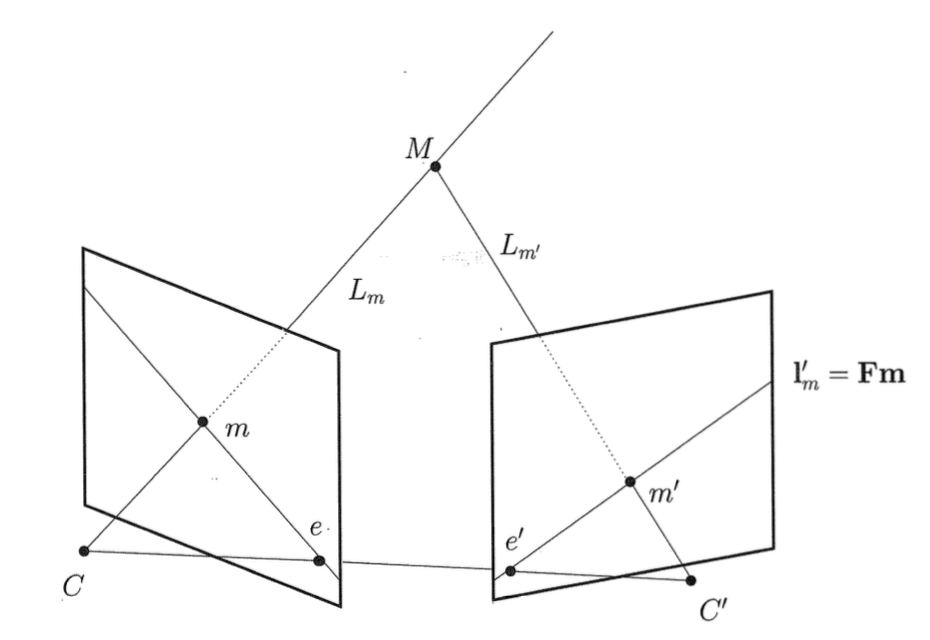
\includegraphics{Imagens/figura2-4.png}
	\caption{Exemplo de geometria epipolar. Dado um ponto $m$, o seu correspondente $m'$ precisa estar na linha epipolar $l'm$. Dada a correspondência válida entre $m$ e $m'$, a interseção dos raios ópticos $Lm$ e $Lm$ é não-vazia, e coplanar com a linha $CC'$. Faugeras et al \cite{Faugeras-Geometry} pag. 25.}
	\label{fig4}
\end{figure}

Normalmente não se assume qualquer relação espacial entre os pontos no espaço, apenas a informação disponível pela correspondência projetiva, ou seja, a correspondência de pontos por projeção linear. A geometria epipolar é a restrição básica que decorre da existência de dois pontos de vista distintos. Ambos podem ser obtidos por duas câmeras diferentes ou com uma câmera em movimento, denominado \textit{Structure from Motion}. As restrições epipolares descrevem totalmente a correspondência de pares de correspondências genéricas entre pontos de cada imagem, e a ambiguidade ao longo da linha epipolar causada pela ambiguidade ao longo dos raios ópticos da operação de projeção. Partindo do fato de que a matriz fundamental depende apenas da geometria da câmera, descreve todas as restrições epipolares, logo compila toda a informação disponível das correspondências projetivas. 

Já que todos os raios ópticos contém o centro óptico $C$ da primeira câmera, todas as linhas epipolares contém a projeção de $C$ na segunda imagem nos pontos onde a primeira câmera é vista pela segunda, chamada epípole. Como mostra a figura \ref{fig2}, o fato da epípole  da segunda imagem pertencer às linhas epipolares significa que $e'TFm = 0$, ou, $FTe' = 0$. Invertendo as duas imagens, $Fe = 0$. Pode-se concluir que $F$ é uma matriz de grau 2 e $det(F) = 0$. Como essa restrição algébrica é satisfeita e é apenas definida por um fator de escala, $F$ depende de sete parâmetros.

Para o cálculo da matriz fundamental, tem-se $m$ e $m'$ correspondentes abaixo:

\begin{equation}\label{eq5}
m = \begin{bmatrix}u\\v\\1\\ \end{bmatrix}
\end{equation}

Equação \eqref{eq5}: Matrizes dos pontos $m$ e $m'$.

e $F$ a matriz fundamental:

\begin{equation}\label{eq6}
F = 
\begin{bmatrix}
	F_{11} &  F_{12} &  F_{13}\\
	F_{21} &  F_{22} &  F_{23}\\
	F_{31} &  F_{32} &  F_{33}
\end{bmatrix}, m' = \begin{bmatrix}u'\\v'\\1\end{bmatrix}
\end{equation}

Equação \eqref{eq6}: Matriz fundamental $F$.

Logo, a restrição epipolar $m'TFm = 0$ pode ser representada como $UTf = 0$, onde:

\begin{equation}\label{eq7}
f = [F_{11}, F_{12}, F_{13}, F_{21}, F_{22}, F_{23}, F_{31}, F_{32}, F_{33}]
\end{equation}
\begin{equation}\label{eq8}
U = [uu', vu', u', uv', vv', v', uv]
\end{equation}
\begin{equation}\label{eq9}
\begin{bmatrix}u' & v' & 1\end{bmatrix} 
\begin{bmatrix}
	F_{11} &  F_{12} &  F_{13}\\
	F_{21} &  F_{22} &  F_{23}\\
	F_{31} &  F_{32} &  F_{33}
\end{bmatrix}
\begin{bmatrix}u\\v\\1\end{bmatrix} = u'
\end{equation}

Equações \eqref{eq7}, \eqref{eq8} e \eqref{eq9}: Representações de $f$, $U$ e $UTf$.

Tal sistema de equações é linear, homogêneo e possui 9 incógnitas, com 8 pares de pontos correspondentes. É possível encontrar uma solução única para $F$ determinam de até um fator de escala, conhecido também como o algoritmo dos 8 pontos.


\section{Algoritmos de detecção de características}

Encontrar estruturas partindo do movimento apresenta problemas também na visão estéreo, onde há duas câmeras sendo utilizadas para obter mais informações sobre um mesmo objeto sob diferentes pontos de vista, mas a correspondência entre as imagens obtidas e os objetos 3D precisam ser encontradas. Para isso, são utilizadas características distintas como cantos e vértices, possuindo também diferentes gradientes em múltiplas direções, de uma imagem para outra. O algoritmo mais conhecido atualmente é o \textit{SIFT} \cite{SIFT}, onde utiliza a máxima para a pirâmide de diferença de \textit{Gauss} como características. Primeiramente o \textit{SIFT} procura uma direção dominante no gradiente, e para deixá-lo invariante à rotação, rotaciona o descritor para que sua orientação seja compatível.

O \textit{SURF}\cite{SURF} também é um algoritmo conhecido na tarefa de obter características, mas ao invés de obter as diferenças de \textit{Gauss}, se baseia em determinantes de matrizes Hessianas para localização e escala \cite{Hessian}. E ao invés de calcular histogramas dos gradientes, computa a soma dos componentes destes com seus valores absolutos. Todas as características detectadas de todas as imagens então são combinadas.

O \textit{ORB (Oriented FAST and Rotated BRIEF)} surgiu como uma alternativa ao algoritmo de detecção e descrição de pontos característicos \textit{SIFT} na questão de eficiência em smartphones, já que se mostra mais eficiente em dispositivos com menos poder de processamento, bem como não ser patenteado, ao contrário do \textit{SIFT} e \textit{SURF}, podendo acarretar em problemas de propriedade intelectual. O \textit{ORB} toma como base a detecção de pontos característicos do \textit{SIFT} e o descritor do \textit{BRIEF}, já que ambos são bem eficientes nestas tarefas e baixo custo computacional. Um dos problemas demonstrados por Rublee et al\cite{ORB-Artigo} em seu artigo é a falta de invariância com relação à rotação no \textit{BRIEF}.

Como dito anteriormente, o algoritmo \textit{FAST} foi escolhido para detecção de \textit{keypoints} em sistemas em tempo real que procuram um casamento isto é, encontrar a similaridade entre duas imagens, entre características visuais, mas o algoritmo precisava ser incrementado com a pirâmide de \textit{schemes} para escala\cite{ORB-Artigo} e o filtro de Harris\cite{ORB-Artigo} para rejeitar cantos. Ao contrário do \textit{SIFT} e \textit{SURF}, o \textit{FAST} não provém de um operador de orientação. Como descrito em seu artigo, há várias formas de se descrever a orientação de um \textit{keypoint}. Algumas destas formas envolvem computações de histogramas de gradientes, mas tais métodos são muito ostensivos computacionalmente e no caso do \textit{SURF}, levando à aproximações não muito boas.

Para os descritores, o \textit{BRIEF} é utilizado pela robustez para luz, \textit{blur} e distorção de perspectiva, mas é sensível com a rotação do plano \cite{ORB-Artigo}. O \textit{BRIEF} utiliza testes binários para treinar um conjunto de árvores de classificação \cite{ORB-Artigo}, normalmente treinadas com 500 ou mais \textit{keypoints}, podem ser utilizadas para retornar a assinatura de um \textit{keypoint arbitrário} \cite{ORB-Artigo}.

Infelizmente as combinações encontradas podem ser errôneas, logo é preciso eliminar falsos positivos. Para isso normalmente se é utilizado o \textit{RANSAC} , algoritmo que remove combinações de pontos \textit{outliers}, isto é, combinações que provavelmente não pertencem ao espaço. O \textit{RANSAC} também é utilizado para resolver o \textit{Location Determination Problem}, que tem como objetivo determinar os pontos no espaço que têm projeção numa imagem com localizações conhecidas \cite{RANSAC}.

As características adquiridas ao longo do tempo são usadas para reconstruir suas localizações no espaço 3D e o movimento da câmera. Outra alternativa são as “abordagens diretas”, que tentam obter as informações geométricas sem abstração intermediária como características ou cantos.


\section{\textit{Simultaneous Localization And Mapping}}

O termo \textit{SLAM} é a sigla para \textit{Simultaneous Localization And Mapping}. O \textit{SLAM} foi criado a partir do problema de construir um mapa de um ambiente desconhecido por um robô móvel enquanto ao mesmo tempo navega pelo ambiente usando o mapa. \textit{SLAM} consiste de múltiplas partes: Extração de pontos de referência, associação de dados, estimativa de estados, e atualização de ponto de referência. Há várias formas de resolver cada uma dessas partes menores que pode ser exclusivo de cada implementação\cite{SLAM-Dummies}. Na abordagem padrão para o \textit{SLAM} usa-se sensores a \textit{laser} para estimar a distancia entre os pontos de referência e fazer o cálculos com base nesses dados. No caso desse trabalho ao invés de \textit{lasers} e sensores de movimento buscou-se métodos para uso de apenas uma câmera em junção com \textit{Computer Vision e Multiple View Geometry} para que essa implementação possa ser usada potencialmente em dispositivos móveis e por pessoas e não robôs. O \textit{LSD-SLAM} oferece essa abordagem usando gradientes de imagens digitais e por ser o método utilizado, será discutido nas próximas sessões.

\section{\textit{LSD-SLAM}}

Um dos maiores benefícios do \textit{SLAM} monocular, e simultaneamente o seu maior desafio, vem da sua ambiguidade de escala inerente: A escala do mundo não pode ser observado e muda com o tempo, sendo uma das maiores fontes de erro. A vantagem é que isso permite a troca entre ambientes de diferentes escalas como ambientes internos com móveis e ambientes externos. Por outro lado sensores escalonados como câmeras estéreo e câmeras de profundidade provém resultados mais confiáveis mas não oferecem a mesma flexibilidade tanto na facilidade de troca entre diferentes escalas quanto no \textit{hardware}, fazendo a abordagem \textit{monocular} funcionar para câmeras de celular que é um \textit{hardware} mais acessível. 

Segundo o artigo do \textit{LSD-SLAM} \cite{LSD-SLAM-Artigo}, o algoritmo consiste de três componentes principais: \textbf{tracking (rastreamento)}, \textbf{depth map estimation (estimativa de mapa de profundidade)} e \textbf{map optimization (otimização de mapa)} :

\begin{itemize}
	\item{O componente de \textbf{tracking} continuamente rastreia novas imagens de câmera; Isso é, ele estima sua pose de corpo rígido $\xi \in se(3)$ com relação ao quadro-chave atual, usando a pose do quadro anterior como inicialização.}
	\item{O componente de \textbf{depth map estimation} usa quadros rastreados para refinar ou repor o quadro-chave atual. A profundidade é refinada filtrando entre várias comparações estéreo de pequeno patamar por \textit{pixel} casada com regularização espacial intervalada. Se a câmera se mover muito longe, um novo quadro-chave é inicializado projetando os pontos de quadros-chave perto já rastreados nele.}
	\item{Assim que o componente do \textbf{depth map estimation} define que a imagem atual não deve ser usada para refinamento, mas como um novo quadro-chave, o anterior é reposto pela nova imagem que se torna um quadro-chave. O mapa de profundidade do quadro chave anterior não será mais refinado e é incorporado ao mapa global pelo componente de \textbf{map optimization}. Para detectar fechamentos de \textit{loops} e mudança de escala uma transformada de similaridade $\xi \in sim(3)$ para \textit{keyframes} já capturados próximos é estimada usando um alinhamento direto de imagem $sim(3)$ que é ciente de escala.}
\end{itemize}